\section{PIV Overview}

Particle image velocimetry (PIV) is a flow measurement technique using a flow 
seed particulate, precisely illumination by a laser, and special cameras which 
take multiple closely spaced pictures of the flow. First, the fluid flow is 
seeded with an aerosolized oil fog, which forms tiny, low mass droplets which 
become well entrained in the air. A laser was broadcast into a very thin sheet 
which illuminates a cross section of the flow, where small inhomogeneities in 
the distribution of seed particles can be seen. Cameras were positioned to take 
pictures of the particulate seed in rapid succession, such that the 
displacement of any particular particle group is just a few pixels in the image 
plane of the camera. By tracking movements of particle groupings through each 
image taken at a specific and precise moments in time, with detailed 
information about the geometry of optical setup, displacements in the pixel 
domain could be mapped into displacements in the real spatial domain. These 
displacements were translated into velocities.

Particle image velocimetry has several advantages and disadvantages over other 
flow measurement techniques. Firstly, PIV is non-invasive, with no solid 
positioning system and sensor probe to create its own wake and influence on the 
flow field. Secondly, PIV can make instantaneous and simultaneous measurements 
of an entire two dimensional surface within a flow field. This can greatly 
reduce uncertainty associated with single point surveys over a flow field where 
variation in time and space require very fine control over temperature, 
humidity, and free stream velocity of the flow field in order to isolate. 
Thirdly, PIV can be scaled to accommodate multi dimensional requirements. One 
camera and laser is sufficient to measure two dimensional velocity 
components in a two dimensional slice of space as in figure 
\ref{fig:mono_piv2}. 
Two cameras and a laser is sufficient to measure three dimensional velocity
components in a two dimensional slice of space as in figure
\ref{fig:stereo_piv2}. With multiple polarized laser beams, it is possible even
to measure three dimensional velocity fields within a volume of space. 

\begin{figure}[H]
	\centering
	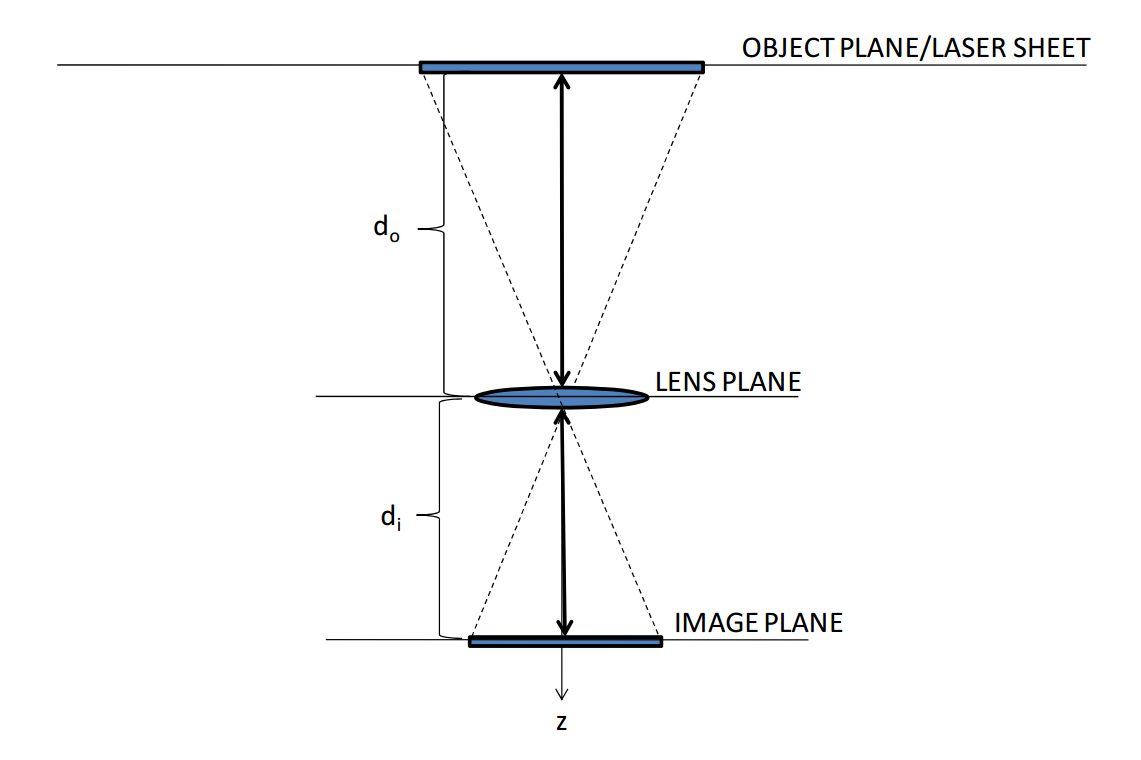
\includegraphics[width=5in]{figs/piv_method/mono_piv_optics}
	\caption{Single camera PIV system for mapping two dimensional velocity 
	vectors}
	\label{fig:mono_piv2}
\end{figure} 


\begin{figure}[H]
	\centering
	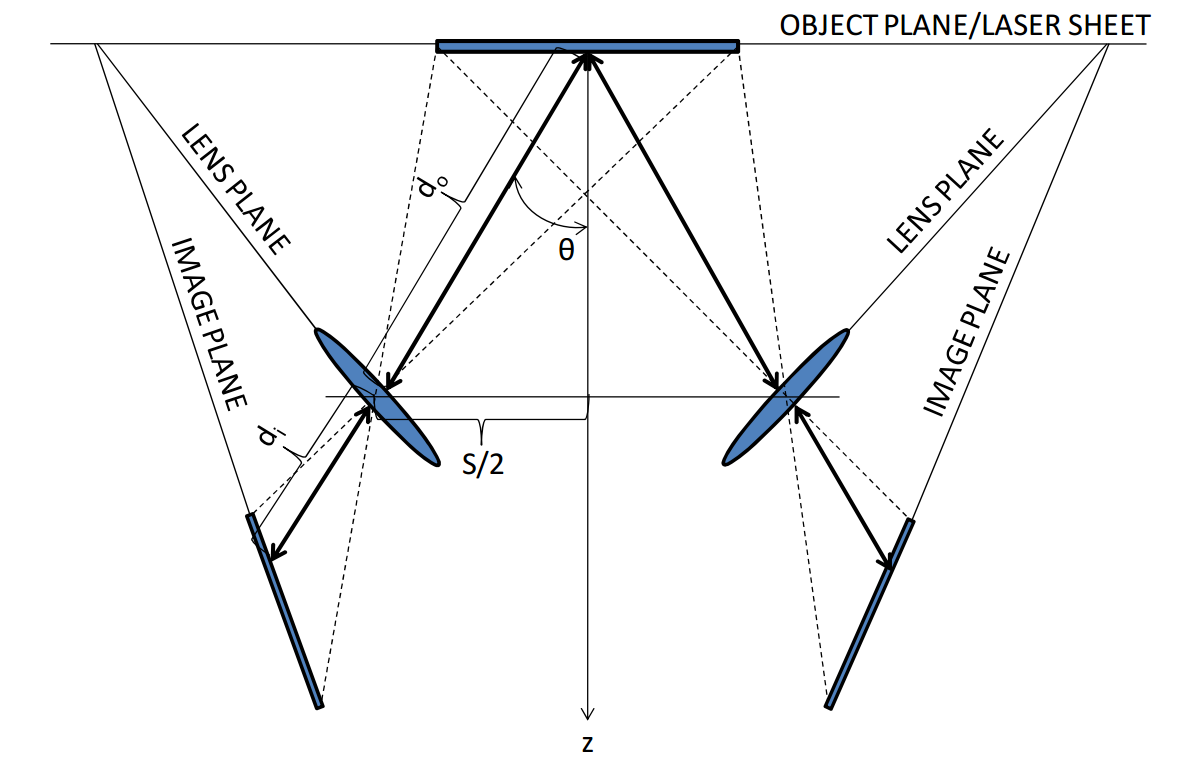
\includegraphics[width=5in]{figs/piv_method/stereo_piv_optics}
	\caption{Stereo camera PIV system for mapping three dimensional velocity 
		vectors}
	\label{fig:stereo_piv2}
\end{figure} 


A significant disadvantage is that the sampling rate is restricted by the 
shutter speed on the cameras, and this shutter speed can easily be slower than 
the time scales at which turbulent phenomena may occur. As technology improves,
this disadvantage is slowly vanishing, as cameras with sampling rates on the
order of 20kHz are becoming available, though at extremely high cost. An
additional disadvantage which also erodes with improved computing power is the
relatively high computational intensity of processing large volumes of raw
image data into fully resolved vector fields, especially at a high sampling
rate.

The present study uses a stereo PIV system which resolves three dimensional 
vectors gridded to a two dimensional cross section of flow. The cameras used 
are capable of taking two images a few microseconds apart, 
but cannot fully open and close the shutter that quickly. Deriving velocity 
vectors requires two images just a few microseconds apart, but pairs of images 
can be taken at greater time intervals. The PIV method used in this study 
relies upon a frame straddling technique, that times laser pulses at the edges 
of the camera exposures in order to meet this requirement. This results in two 
cameras, which simultaneously take a pair of images, and 25-50 microseconds 
later take a second pair of snapshots for a total of four images, $Ra$, $Rb$, 
$La$, and $Lb$. This can be repeated once every second, resulting 
in a true sampling frequency of 1Hz.

\subsection{Seeding the Flow}

Appropriate particle seeding density and time between straddled frames is the
subject of continued study, and is difficult to predict before hand. 
Completeness of a two dimensional vector field is highly dependent upon 
uniform optimal particle density conditions which are difficult to obtain, and 
maintain over an extended test. For stereo PIV, incomplete data in either of 
the two dimensional vector 
sets from either camera at a given spatial location will result in an 
indeterminate vector displacement in the three dimensional vector data. To 
elevate the likelihood that a displacement vector at a given location can be 
properly determined, an additional data refining technique outlined in Hart 
(flag, reference) was employed. The Hart method compares correlation maps 
between two adjacent sectors for consistency. in instances where two adjacent 
regions lack a well-defined peak, the Hart method functions to magnify shared 
peaks and reveal a solution that might otherwise have been missed. In instances 
where sub optimal seeding conditions were present and a correlation map 
produces a false peak, the Hart method functions to rule the peak out as an 
anomaly if the adjacent sectors do not also indicate a high correlation at that 
location \cite{hart1998}. The way in which in which the Hart method reduces the 
number of erroneous vectors present in a data set is difficult to quantify on a 
case by case basis, but any impact on overall uncertainty of the PIV 
measurements is expected to have a reducing effect.